\subsection{Metrics for Performance Evaluation}
\label{sec:neural-networks-metrics}
There are several common metrics available that, for example, measure the classification accuracy or its precision.
However, they depend on some definitions that will be introduced first.
The positive class of a data sample represents its ground-truth class, while the negative one represents any of the remaining ones, i.\,e. not the positive class.
A true positive $TP$ is a correct prediction of a sample, so the positive class is predicted correctly.
A true negative $TN$ is a correct rejection of a sample, i.\,e. the network classifies this sample correctly as not the positive class.
Furthermore, a false positive $FP$ is a wrong prediction of a sample as the positive class.
The last definition is a false negative $FN$.
This means the network incorrectly predicts a sample as a negative class.
Their connection is visualized in \figref{fig:confusion-matrix} showing the so-called confusion matrix \cite{Fawcett:2006:IRA:1159473.1159475} for the example class Class A.
This needs to be repeated for each class in a dataset.
\begin{figure}
	\centering
	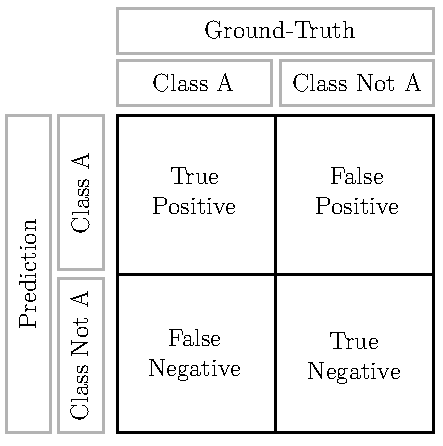
\includegraphics[]{images/confusion_matrix.pdf}
	\caption[Confusion matrix]{Confusion matrix for class A.}
	\label{fig:confusion-matrix}
\end{figure}
One metric is the accuracy
\begin{equation}
	ACC = \frac{TP + TN}{TP + TN + FP + FN}
\end{equation}
of a class.
Averaging all class accuracies yields the network accuracy.
This states how many samples the network correctly classifies.
However, this metric's results are not reliable for the real performance, because it highly depends on the dataset and its balance, among others.
If it is unbalanced there are, for example, more samples in a well-classifiable class than in a bad one, hence, the accuracy is shifted.
The precision or positive predicted value of a class measures how accurate the related predictions are and is calculated by
\begin{equation}
	\label{eq:metric-precision}
	PPV = \frac{TP}{TP + FP}
\end{equation}
where the denominator refers to the total positive results.
Furthermore, the recall or true positive rate metric measures how good all positives of a class are found by
\begin{equation}
	\label{eq:metric-recall}
	TPR = \frac{TP}{TP + FN}
\end{equation}
where the denominator refers to the actual positives of a class.
Both \eqref{eq:metric-precision} and \eqref{eq:metric-recall} must be calculated for each class to get a complete overview of the dataset.
A simplified representation of the confusion matrix can be prepared by entering only the number of predictions per class.
This is beneficial for a quick overview of the prediction distribution of multi-class classifications.
Similar to \figref{fig:confusion-matrix} each row represents a predicted class, while the columns represent the ground-truth classes.
Each prediction of the samples of a ground-truth class are summed per class and entered at the corresponding cell.